% -*- mode: latex; coding: latin-1-unix -*- %

\subsection{Comparaison}

\begin{frame}
\frametitle{Arbre 5 sommets}
\begin{center}
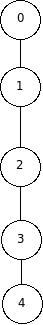
\includegraphics[scale=0.6]{arbre5sommets}
\end{center}
\end{frame}

\begin{frame}
\frametitle{Comparaison entre l'algorithme optimal et l'algorithme 2-approch�}
\begin{block}{Sur un arbre � 5 sommets - Temps d'execution}
  \begin{itemize}
  \item Algorithme optimal : 0,016 secondes
  \item Algorithme 2-approch� : 0,003 secondes
  \end{itemize}
\end{block}
\begin{block}{Sur un arbre � 5 sommets - R�sultats}
  \begin{itemize}
  \item Algorithme optimal : 1 3
  \item Algorithme 2-approch� : 1 3
  \end{itemize}
\end{block}
\end{frame}


\begin{frame}
\frametitle{Arbre 9 sommets}
\begin{center}
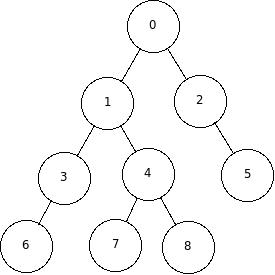
\includegraphics[scale=0.7]{arbre9sommets}
\end{center}
\end{frame}

\begin{frame}
\frametitle{Comparaison entre l'algorithme optimal et l'algorithme 2-approch�}
\begin{block}{Sur un arbre � 9 sommets - Temps d'execution}
  \begin{itemize}
  \item Algorithme optimal : 0,013 secondes
  \item Algorithme 2-approch� : 0,006 secondes
  \end{itemize}
\end{block}
\begin{block}{Sur un arbre � 9 sommets - R�sultats}
  \begin{itemize}
  \item Algorithme optimal : 1 2 3 4
  \item Algorithme 2-approch� : 0 2 3 4
  \end{itemize}
\end{block}
\end{frame}


\begin{frame}
\frametitle{Arbre 15 sommets}
\begin{center}
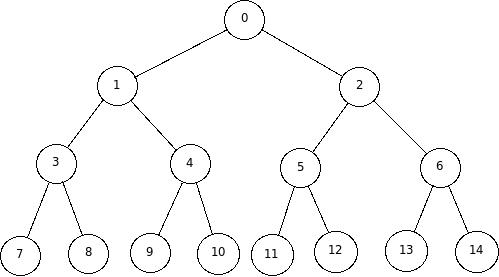
\includegraphics[scale=0.6]{arbre15sommets}
\end{center}
\end{frame}

\begin{frame}
\frametitle{Comparaison entre l'algorithme optimal et l'algorithme 2-approch�}
\begin{block}{Sur un arbre � 15 sommets - Temps d'execution}
  \begin{itemize}
  \item Algorithme optimal : 0,030 secondes
  \item Algorithme 2-approch� : 0,007 secondes
  \end{itemize}
\end{block}
\begin{block}{Sur un arbre � 15 sommets - R�sultats}
  \begin{itemize}
  \item Algorithme optimal : 0 3 4 5 6
  \item Algorithme 2-approch� : 0 3 4 5 6
  \end{itemize}
\end{block}
\end{frame}

\begin{frame}
\frametitle{Graphe 20 sommets}
\begin{center}
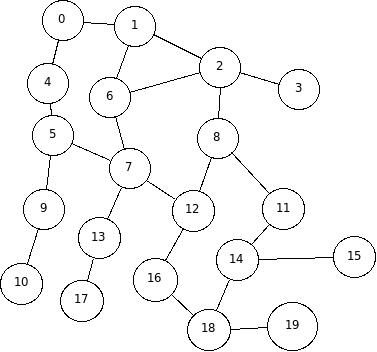
\includegraphics[scale=0.6]{graphe20sommets}
\end{center}
\end{frame}

\begin{frame}
\frametitle{Comparaison entre l'algorithme optimal et l'algorithme 2-approch�}
\begin{block}{Sur un graphe � 20 sommets - Temps d'execution}
  \begin{itemize}
  \item Algorithme optimal : 0,028 secondes
  \item Algorithme 2-approch� : 0,006 secondes
  \end{itemize}
\end{block}
\begin{block}{Sur un graphe � 20 sommets - R�sultats}
  \begin{itemize}
  \item Algorithme optimal : 1 2 4 7 8 9 13 14 16 19 (10 sommets)
  \item Algorithme 2-approch� : 0 1 2 5 7 8 9 11 12 13 14 16 18 (13 sommets)
  \end{itemize}
\end{block}
\end{frame}

\begin{frame}
\frametitle{Comparaison entre l'algorithme optimal et l'algorithme 2-approch�}
\begin{block}{Sur un graphe � 40 sommets - Temps d'execution}
  \begin{itemize}
  \item Algorithme optimal : 0,078 secondes
  \item Algorithme 2-approch� : 0,008 secondes
  \end{itemize}
\end{block}
\begin{block}{Sur un graphe � 40 sommets - R�sultats}
  \begin{itemize}
  \item Algorithme optimal : 34 sommets
  \item Algorithme 2-approch� : 37 sommets
  \end{itemize}
\end{block}
\end{frame}

\begin{frame}
\frametitle{Comparaison entre l'algorithme optimal et l'algorithme 2-approch�}
\begin{block}{Sur un graphe � 100 sommets - Temps d'execution}
  \begin{itemize}
  \item Algorithme optimal : 0,268 secondes
  \item Algorithme 2-approch� : 0,015 secondes
  \end{itemize}
\end{block}
\begin{block}{Sur un graphe � 100 sommets - R�sultats}
  \begin{itemize}
  \item Algorithme optimal : 95 sommets
  \item Algorithme 2-approch� : 99 sommets
  \end{itemize}
\end{block}
\end{frame}


\subsection{Instance Critique}

\begin{frame}
\frametitle{Instance N�gative}
\begin{block}{Bilan du projet XP}
  \begin{itemize}
  \item Projets r�utilisant du code, non adapt�s � XP
  \item Code fourni peu document�
  \end{itemize}
\end{block}
\end{frame}
